\section{JavaCard Firmware}\label{impl:firmware}
The Trusted Execution Module architecture proposed in chapter \ref{arch} was
implemented on top of the JavaCard architecture. The platform was ``chosen''
because I could not obtain a development kit for any other secure
chip, at a reasonable price.

The JavaCard platform is implemented on smartcard chips that conform to the
ISO 7816 standard. Using JavaCard translated into fast development, and the
satisfaction of being able to show off my TEM inside a real chip.

\subsection{Overall Design}
The firmware's overall design closely reflects the TEM architecture illustrated
in figure \ref{fig:tem_overview}\footnote{Or, perhaps the  architecture reflects
the firmware design.}. Each architecture component was implemented as a class
consisting of \texttt{static} fields and methods. JavaCard supports object
creation, and that would have made the syntax a bit less clunky. However, the
the runtime overhead of objects was not warranted, given that all I needed were
namespaces and encapsulation.

\subsection{Memory Management: the Buffer Pool}
The desktop Java platform automates memory management. JavaCard restores some
of the control to the applications, for maximum performance. Objects are still
garbage collected, but the application controls when that happens. More
importantly, the application is responsible for deciding whether an object is
stored into RAM or EEPROM memory.

The sensible strategy of choosing the memory type based on an object's need to
survive does not work, because JavaCard smart cards have very little
available RAM (about 2KB) and significantly more EEPROM (our models have between
18KB and 72KB). Deciding which objects go into RAM impacts performance (RAM is
faster than EEPROM) and the card's lifetime (EEPROM wears out after a finite
number of write cycles, RAM does not).

The buffer pool uses heuristics to determine the memory that an object should go
to. The heuristics are currently based on the requested buffer size and the
amount of free memory. Buffers are marked (pinned) when they are in use, so the
memory manager can move buffers that are not used between RAM and EEPROM, to
improve utilization.

\subsection{Communication Interface: the Applet}
The ISO 7816 standard establishes the APDU (Application Protocol Data Unit) as
the packet in the communication protocol between a smartcard and its host. The
standard also specifies that smart cards process commands synchronously, by
repeating the following loop: receive a command APDU, execute the command,
reply with a response APDU.
 
The communication interface in the TEM architecture (section
\ref{arch:interface}) is implemented by a subclass of the
\texttt{javacard.framework.Applet} class. The applet subclass is invoked when
the smart card receives a command APDU, and is responsible for decoding the
command, invoking the appropriate engine, and returning the result.

APDUs are limited to 255 bytes, out of which 5 bytes are used as a header.
SECpacks exceed this limit\footnote{The Endorsement Key is a 2048-bit RSA key,
so $\mathcal E$ in a bound SECpack is at least 256 bytes.}, so the command APDU
that says ``load a SECpack'' must deal with fragmented SECpacks. To avoid
repeating this pattern, the applet provides APDUs for allocating buffers, and
then reads from / writes to them using multiple commands. Buffer IDs are
used instead of parameters and return values in command or response APDUs.

\subsection{Virtual Machine Interpreter}
The TEM's VM interpreter is implemented as one single 420-line method, most of
which is one big \texttt{switch} statement. This contrasts with the rest of the
TEM implementation, which is rather modular, and is definitely a departure from
OOP software engineering principles.

The unusual implementation was chosen because there was a single developer
(myself) working on the code, and it was clear that the code would change a lot
as I gained more experience by writing more closures. The consistency in the
TEM's instruction set (section \ref{arch:vm_instructions}), together with the
freedom of defining the opcode table, were used to build very tight code.
For example, all the jump operations are implemented by the code in listing
\ref{impl:interpreter_jumps}. The meat of the code is about 10 lines, and
everthing else is ``fat'' introduced by Java's lack of support for ranges as
case labels.

\lstinputlisting[float=bph, language=Java, caption=VM Interpretor Code for
Conditional Jumps, label=impl:interpreter_jumps]{code/vm_interp_jumps.java}

The instruction mnemonics included in the comments are used to facilitate
navigation in the interpreter code, by serving as targets for the \textit{Find}
command in any IDE.

\subsection{SEClosure Execution}
The TEM's synchronous excution model fits \textit{almost} well with the ISO
7816 command-response protocol, so it seems that the interface to the
execution engine should consist of a single APDU, \textit{load and execute
SECpack} . The harmony breaks when closures invoke persistent store operations,
and the TEM on the smart card needs to exchange messages with the host computer
before the \textit{load and execute} command is completed.

My solution to this problem was to model the execution engine as the state
machine illustrated in figure \ref{fig:exec_states}. Each state is a
transaction. When a persistent store operation occurs, the VM interpreter's
state is saved, and execution is suspended. Once the persistent store
fault\footnote{think page fault} is resolved by reading or modifying the correct
association from the persistent store (section \ref{arch:pstore_external}),
execution is resumed using the saved state. Having a stack-based VM interpreter
makes saving its state really easy -- the state is completely described by the
Instruction Pointer (IP), Stack Pointer (SP), and the number of bytes written in
the append-only output buffer (Output Pointer - OP). 

\begin{figure}
	\center{
		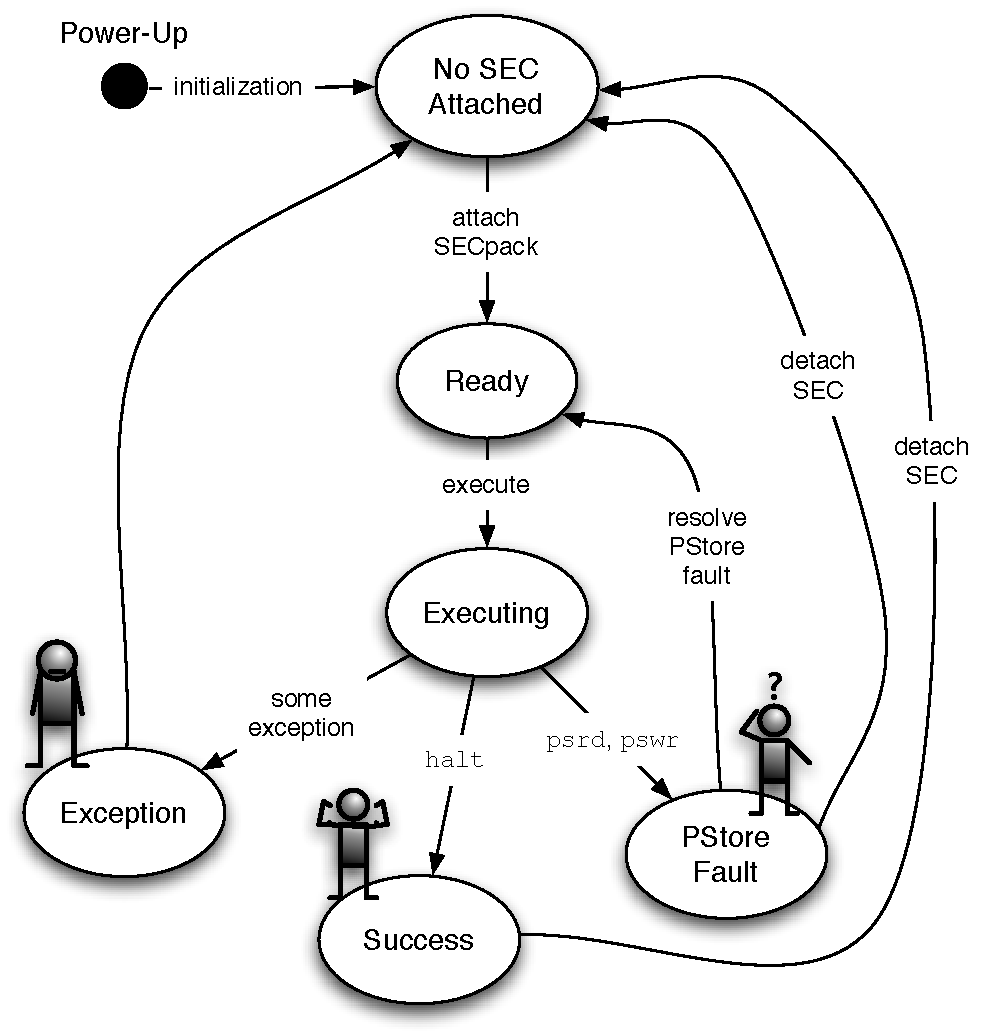
\includegraphics{omnifigs/execution_states}
	}
	\caption{State Machine for the TEM's Execution Engine}
	\label{fig:exec_states}
\end{figure}


\subsection{Development Support}\label{impl:fw_dev_support}
The prototype TEM implementation contains supplemental features to help
debugging SEClosures. These features are usually associated with ``developer
versions'' of chips.

When an exception occurs, the state of the VM interpreter is saved, using the
same code path as for persistent store faults. Detaching an exception-causing
SEClosure from the execution engine returns the interpreter state to the driver
software. The prototype driver implementation uses the information to show the
user the line of code containing the VM instruction that caused the exception.
Section \ref{impl:driver_dev_support} describes the driver side of the
mechanism and shows a processed SEClosure execution exception.

The prototype TEM is also capable of producing a list of the buffers
allocated by the memory managers, as well as a list of the keys in the
persistent store. This information is also processed by the prototype driver,
producing the snapshot shown in section \ref{impl:driver_dev_support}.

In order to ensure that the development features do not interfere with a
closure's confidentiality requirements, the SECpack header contains a flag that
indicates if development support features are allowed to be used with that
SECpack.

\subsection{Performance Considerations}
The table below shows the results of various tests that were run on two
JavaCard models. The times are expressed in seconds, and are averaged over
multiple repetitions of each operation. The number of repetitions was chosen
such that the results of running an experiment 3 times were within 1\% of the
mean.

\begin{center}
\begin{tabular}{|l|r|r|}
\hline
\textbf{Operations} & \textbf{NXP 41/72k} & \textbf{Philips 21 18k} \\
\hline
Process APDU & 0.0061 s & 0.029 s \\
\hline
Create and release 512-byte buffer & 0.084 s & 0.98 s \\
\hline
Decrypt with PrivEK & 0.76 s & 1.60 s \\
\hline
Execute 1-op SECpack & 0.16 s & 0.50 s \\
\hline
Execute 1020-ops SECpack & 0.82 s & 1.99 s \\
\hline
Execute 1-op bound SECpack & 0.89 s & 1.92 s \\
\hline
Execute 1020-ops bound SECpack & 1.53 s & 3.07 s \\
\hline
\end{tabular}
\end{center}

The SECpack execution performance is nothing to write home about, because
implementing the TEM's execution engine in JavaCard translates to writing a
virtual machine on top of another virtual machine. Usually, the speed difference
between native and interpreted code is on the order of 20X, so it is fair to
assume that a native implementation of the TEM's VM interpreter will be able
to process SECpack instructions an order of magnitude faster.

Despite the overhead introduced by the Java VM, the TEM was able to execute
SEClosures fast enough to make the demos described in section \ref{impl:demos}
work. This is a promising result which reinforces the point that most of a
SEClosure's execution time is spent on cryptographic operations that are
implemented in hardware and do not incur any VM-related overhead.
